% !TEX root = paper.tex

\section{Handling Unsafe Code Safely} \label{sec:unsafe}

Unsafe code can often be a sticking point for users seeking strong guarantees about
their Rust program, as it has the potential to undermine Rust's famous memory-safety guarantees.
In particular, the Rust language guarantees that
a program that does not use \texttt{unsafe} code must unconditionally be memory-safe;
however, when \texttt{unsafe} code is used, the program becomes \emph{conditionally memory-safe};
i.e., the program is only memory-safe if the program obeys certain rules when using
\texttt{unsafe}.

Verus supports a few trusted primitives that are conditionally memory-safe in this manner.
For these cases,
their correctness conditions are encoded as Verus specifications.
Therefore, users can be sure that their code is truly memory-safe (in addition to
\verus' other guarantees) as long as \verus' SMT verification proves that the code upholds
the contracts.

As a simple example, consider the operation of indexing into a vector: one of the most ubiquitous
operations in all of software, yet also one of the most fraught for memory-safety violations.
In Rust, indexing into a vector always performs a bounds check; it is memory-safe because
it will always panic rather than access memory-out-of-bounds.
On the other hand, Rust's \verb`get_unchecked` does not perform any bounds check, and
therefore it an \verb`unsafe` function. That is, \verb`get_unchecked` is conditionally
memory-safe because it is only safe if the user calls the function with a valid index.

We can write this condition as a \verus specification, and provide \verb`get_unchecked`
as a trusted primitive function:

\begin{center}
\begin{lstlisting}[language=Verus,style=VerusLineNos]
fn safe_get_unchecked<V>(v: &Vec<V>, i: usize) -> &V {
    requires 0 <= i && i < v.len()
    ...
}
\end{lstlisting}
\end{center}

In the next sections, we will see some more advanced examples.

\section{Safe Pointer Manipulation with Linear Ghost Types} \label{sec:linear-ghost}

\subsection{Low-Level Pointer Manipulation with Linear Ghost Permissions}\label{sec:ghost:perms}

While Rust's reference types and borrowing rules provide a memory-safe framework for
many use cases, they are sometimes insufficiently expressive and
\emph{raw pointers} may be required.
For example, a doubly-linked list, where each node may be pointed to by two neighbors,
violates the unique-ownership discipline of Rust. Raw pointers are one way to work around
this, although dereferencing raw pointers in Rust requires \verb`unsafe` code.
\verus supports raw (heap) pointers.
The most notable aspect of this support is that,
in order to provide a specification to enforce memory safety, we need to make use of 
linear ghost state.

Specifically, \verus %utilizes its support to track ownership of \verb`proof`-mode objects.
introduces a core primitive
\verb`PPtr<T>` (``permissioned pointer'') as a zero-cost alternative
to raw heap pointers, along
with an associated type \verb`PermData<T>` (``permission plus data'') which is to be used in \verb`proof` mode, i.e., they are linear ghost objects as discussed in the previous section.
Calls to the \verb`PPtr<T>` API require ownership of this ghost permission
object in order to dereference the pointer, which prevents data races and other
forms of access that are undefined behavior in Rust's memory model.

However, the \verb`PermData<T>` object does not ``just'' have the role of maintaining memory safety;
it also tracks the data behind the pointer.
Tracking permissions and data this way lets us write proofs in a style similar to that of separation logics.
Specifically, the permissions object has two fields. The first, \verb`perm.view().pptr`,
indicates the pointer that the permission object corresponds to,
and the second, \verb`perm.view().value`,  gives the data behind the pointer.
The value field is an \verb`Option<T>`,
where a value of \verb`Some(v)` means the memory stores \verb`v`,
and a value of \verb`None` indicates that the memory is uninitialized.
(This should not be confused for the \emph{runtime
representation} of an \verb`exec`-mode \verb`Option<T>`, where \verb`None` is a legitimate, initialized value.)

\autoref{fig:pptr:api} shows two key functions from the \verb`PPtr` API: a function to write
through the pointer (\verb`write`) and a function to read through it (\verb`read`).
Both functions require that the permission is actually associated with the 
pointer being dereferenced~\clref{clnum:pptr:write:requiresid}~\clref{clnum:pptr:read:requiresid}
and \verb`read` requires that the memory being read from
is in an initialized state~\clref{clnum:pptr:read:requiresinit}.
Meanwhile, \verb`write`'s postcondition~\clref{clnum:pptr:write:ensuresvalue} says that the updated permission object
contains the written value, while \verb`read`'s postcondition~\clref{clnum:pptr:read:ensuresvalue} says that the returned value
is the value tracked via the permission.
\autoref{fig:pptr:ex} illustrates the usage of \verb`write` and \verb`read`,
together with allocation and deallocation, showing how the permission \verb`value` is updated.

It is crucial that the \verb`proof`-mode object \verb`PermData<T>` 
obeys Rust's ownership rules.
For example, \autoref{fig:pptr} shows how this prevents a use-after-free bug.
When we free the pointer's memory~\clref{clnum:pptr:example:consume},
the \verb`perm` variable is consumed. Thus Rust's linearity checker would report an error 
if the code attempted to read the pointer
again~\clref{clnum:pptr:example:bad-read}, as this produces another use
of \verb`perm`. 


\begin{figure}

\begin{subfigure}[c]{.46\textwidth}


\begin{lstlisting}[language=Verus,style=VerusLineNos]
impl<T: Copy> PPtr<T> {
    // Equivalent of `*ptr = v`.
    #[exec] pub fn write(&self,
            #[proof] perm: &mut PermData<V>, v: V) {
        requires(equal(self.id(), old(perm).view().pptr)); %*\clnum\label{clnum:pptr:write:requiresid}*
        ensures([
            equal(perm.view().pptr, self.id()),
            equal(perm.view().value, Option::Some(v)), %*\clnum\label{clnum:pptr:write:ensuresvalue}*
        ]);
        ...
    }

    // Read through the pointer and return the value. Requires the memory to be initialized.
    #[exec] pub fn read(&self,
            #[proof] perm: &PermData<V>) -> V {
        requires([
            equal(self.id(), perm.view().pptr), %*\clnum\label{clnum:pptr:read:requiresid}*
            perm.view().value.is_Some() ]); %*\clnum\label{clnum:pptr:read:requiresinit}*
        ensures(|v: V| equal(Option::Some(v),
            perm.view().value)); %*\clnum\label{clnum:pptr:read:ensuresvalue}*
        ...
    }
}
\end{lstlisting}
\caption{Selected functions from the \texttt{PPtr<T>} API, a core \verus primitive.} \label{fig:pptr:api}
\end{subfigure}
\hfill
\begin{subfigure}[c]{.50\textwidth}


\begin{lstlisting}[language=Verus,style=VerusLineNos]
fn main() {
    // Allocate memory.
    let alloc = PPtr::<u64>::empty();
    // Unpack the return value into the pointer and the (ghost) permission
    let pptr = alloc.0;
    #[proof] let mut perm = alloc.1.0;

    // Initially, pptr points to unitialized memory, and the `perm` proof-object represents that as the value `None`.
    assert(equal(perm.view().pptr, pptr.id()));
    assert(equal(perm.view().value, Option::None));

    // We can write a value through the pptr (thus initializing the memory).
    pptr.write(&mut perm, 5); 

    // Having written the value, this is reflected in the permission object:
    assert(equal(perm.view().value, Option::Some(5)));

    // We can now read it:
    let x = pptr.read(&perm); 
    assert(x == 5);

    // Free the memory:
    pptr.free(perm); %*\clnum\label{clnum:pptr:example:consume}*

    // This would error as `perm` was just consumed 
    // let z = pptr.read(&perm); %*\clnum\label{clnum:pptr:example:bad-read}*
}
\end{lstlisting}
\caption{Example usage of \texttt{PPtr<T>}} \label{fig:pptr:ex}
\end{subfigure}
    \caption{
        \label{fig:pptr}
        The \texttt{PPtr<T>} API and an example usage.
        Though the two functions shown here require \texttt{T: Copy}, this is not a general
        restriction on the \texttt{PPtr} library.
    }
\end{figure}


Finally, observe that the safety of this API depends crucially on our ability to add
preconditions (and validate them via the prover).
For example, we saw that the specification of \verb`write` requires that the permission correspond to
the pointer being written through~\clref{clnum:pptr:write:requiresid}, and without this requirement,
it would be wildly unsound.
Thus, a safe API like this is \emph{not possible to implement in vanilla Rust}:
in order to be unconditionally safe,
the precondition would need to be a run-time check,
which would mean the \verb`PermData` object could not be ghost, and the abstraction
could not be zero-cost.

\subsection{Verified Example: Doubly-Linked List} \label{sec:dlist}
Rust's ownership model typically forces data structures to be acyclic,
unless they use unsafe code.
Here, we illustrate how \verb`PPtr` can be used to verify data structures that have cyclic 
pointer arrangements by verifying a double-ended queue implemented with a doubly-linked list.
Specifically, we use a doubly-linked list to represent a sequence $v_0, v_1, \ldots, v_{n-1}$,
and we implement the four operations
$\{\text{\texttt{push}}, \text{\texttt{pop}}\}
\times
\{\text{\texttt{front}}, \text{\texttt{back}}\}$.
The $i$th node in the list has both a \verb`prev` and \verb`next` pointer alongside
a single element of the sequence, $v_i$. The top level datatype, \verb`DList`, contains
\verb`head` and \verb`tail` pointers, pointing to the first and last nodes, respectively.
The full version (which can be found in our supplementary materials~\cite{verussupplementary})
contains an additional space-saving optimization,
where each node does not store its two pointers separately, but rather, stores their bitwise XOR.

\begin{figure}
    \begin{subfigure}{.48\textwidth}
      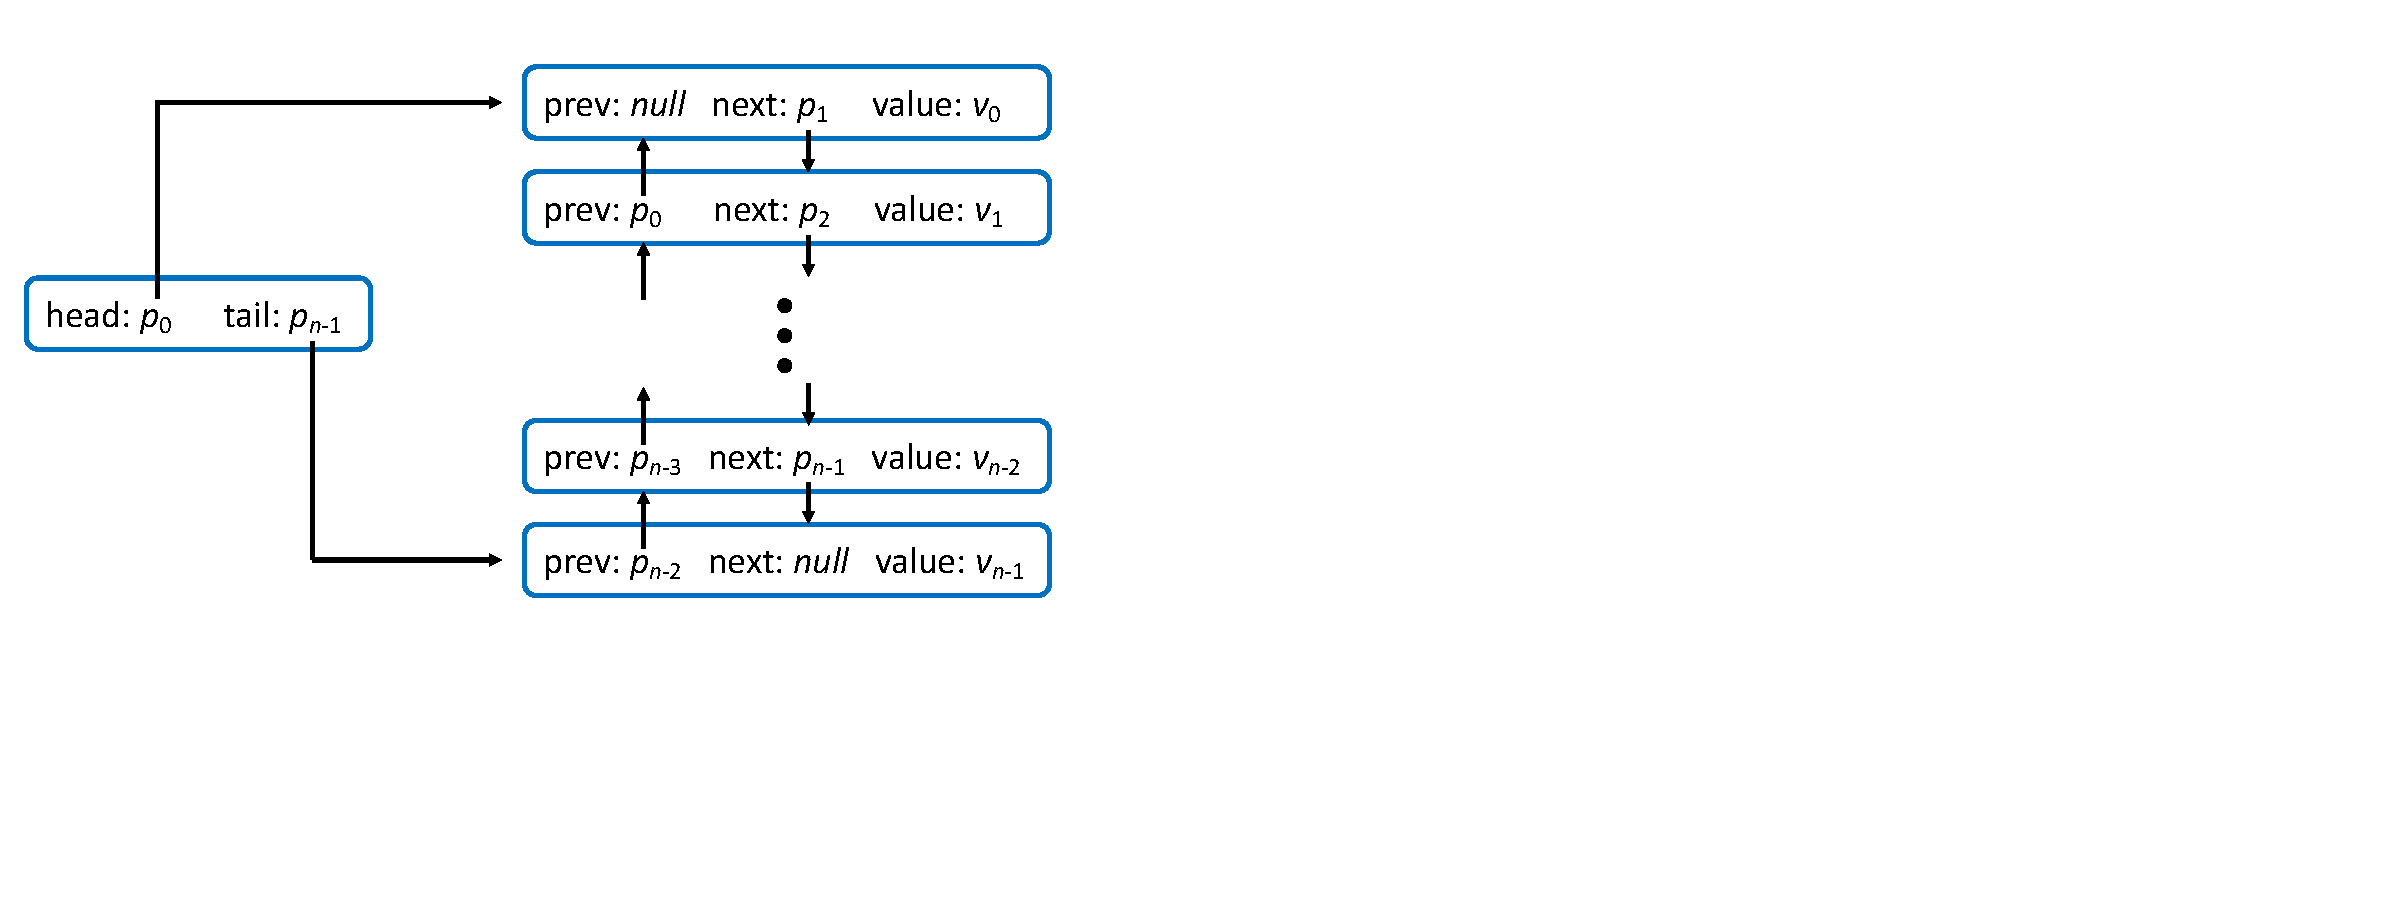
\includegraphics[width=\textwidth]{dlist-diagram-left.pdf}
      \caption{Physical pointer structure of a doubly-linked list.} \label{fig:dlist:phys}
    \end{subfigure}
    \hfill
    \begin{subfigure}{.48\textwidth}
      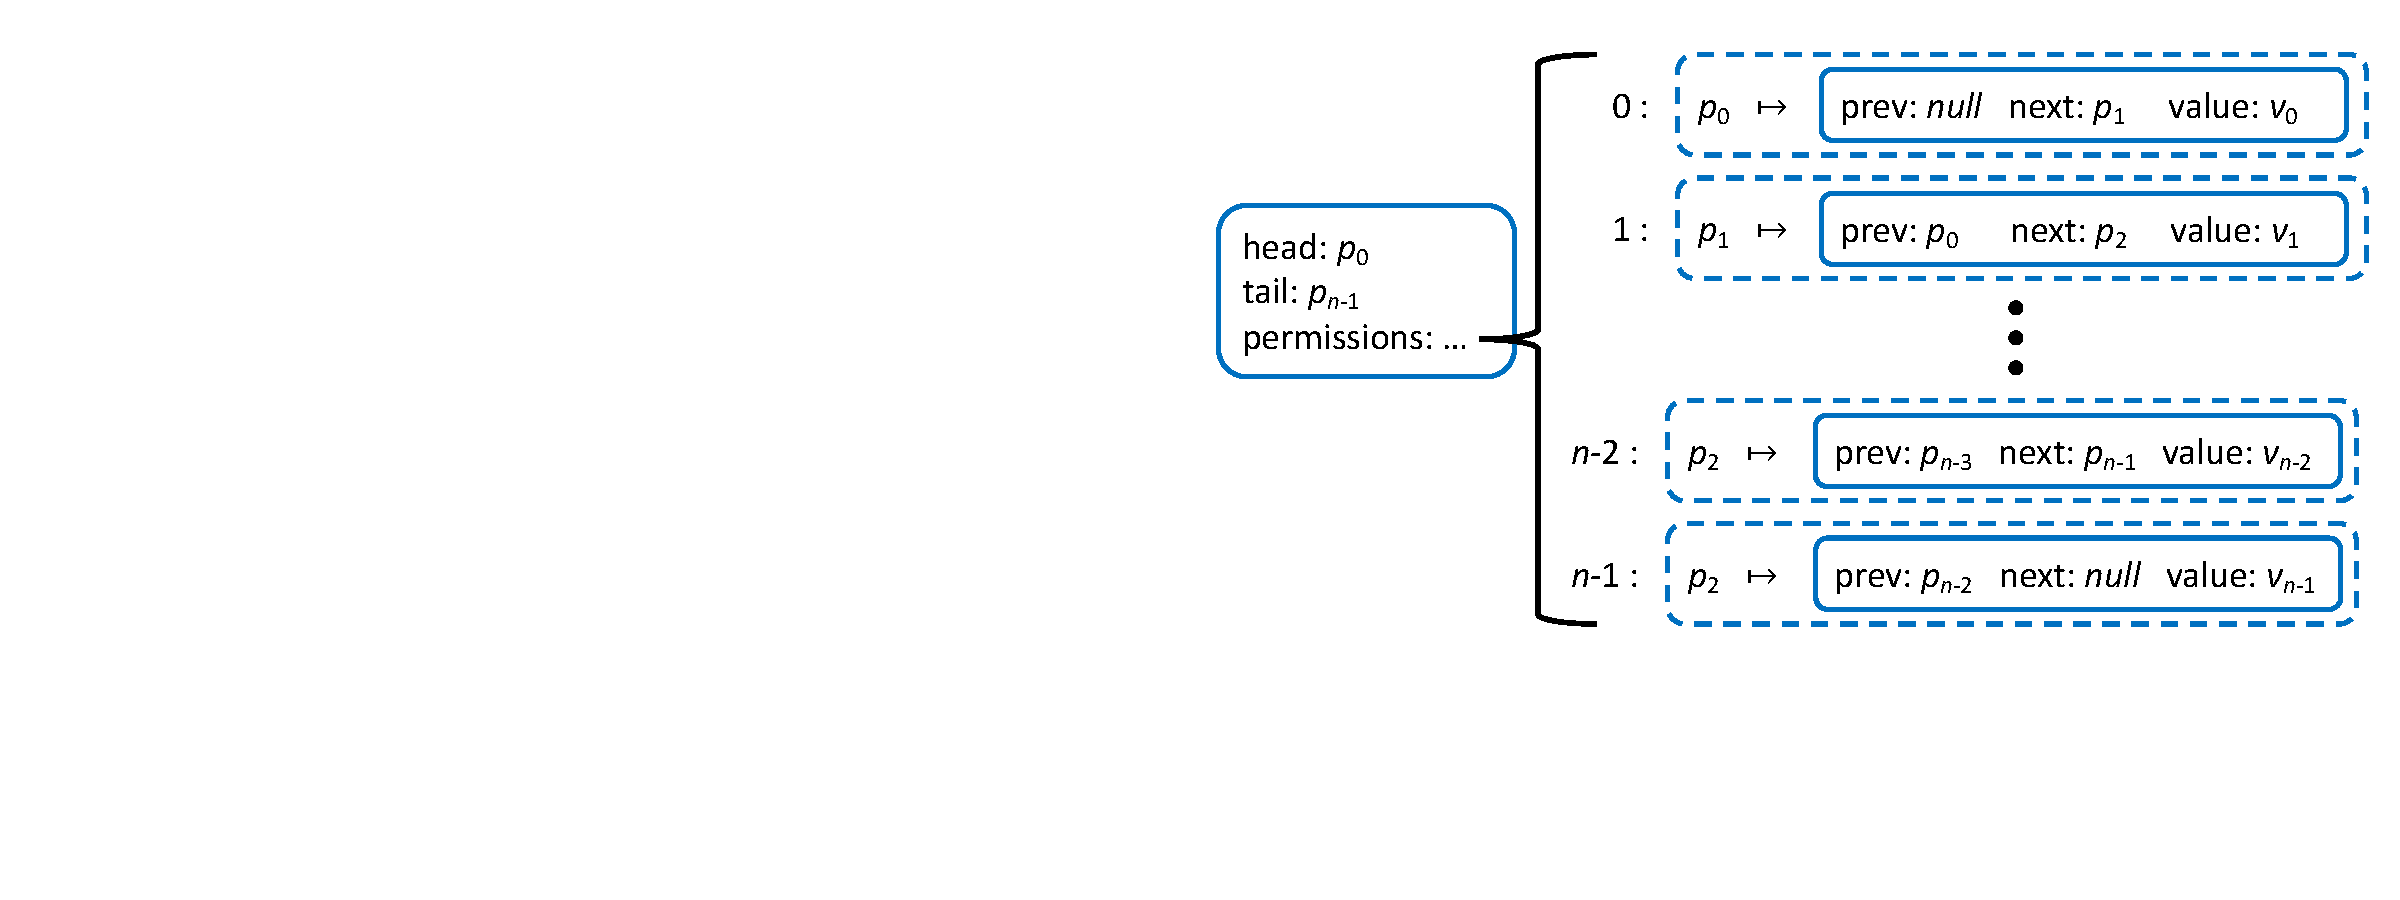
\includegraphics[width=\textwidth]{dlist-diagram-right.pdf}
      \caption{Ownership structure of a \verus doubly-linked list, which includes ghost state.} \label{fig:dlist:ghost}

    \end{subfigure}
    \caption{Doubly-linked lists. The dashed boxes are ghost, \texttt{proof}-mode \texttt{PermData} objects.} \label{fig:dlist}
\end{figure}

\begin{figure}

\begin{subfigure}{.48\textwidth}
\begin{lstlisting}[language=Verus,style=VerusLineNos]
struct Node<V> {
    prev: Option<PPtr<Node<V>>>,
    next: Option<PPtr<Node<V>>>,
    value: V,
}

struct DList<V> {
    #[spec] ptrs: Seq<PPtr<Node<V>>>,
    #[proof] perms: Map<nat, PermData<Node<V>>>,
    #[exec] head: Option<PPtr<Node<V>>>,
    #[exec] tail: Option<PPtr<Node<V>>>,
}

impl<V> DList<V> {
    #[spec] fn view(&self) -> Seq<V> { /* ... */ }

    #[exec] fn new() -> Self {
        ensures(|s: Self| s.well_formed(),
            && s.view().len() == 0); %*\lclnum\label{clnum:dlist:new}*
        /* ... */
    }

    #[exec] fn push_back(&mut self, v: V) {
        requires(old(self).well_formed());
        ensures(self.well_formed() && %*\lclnum\label{clnum:dlist:push-back}*
            equal(self.view(), old(self).view().push(v)));
        /* ... */
    }

    /* push_front, pop_back, pop_front similar */
}

fn main() {
    let mut t = DList::<u32>::new();
    t.push_back(2);   // 2
    t.push_back(3);   // 2, 3
    t.push_front(1);  // 1, 2, 3
    let x = t.pop_back();  // returns 3
    let y = t.pop_front(); // returns 1
    let z = t.pop_front(); // returns 2
    assert(x == 3);
    assert(y == 1);
    assert(z == 2);
}
\end{lstlisting}
\caption{Definition of the \texttt{DList} struct for the doubly-linked list example,
        along with the double-ended queue API, and example usage.} \label{fig:dlist:code:defn}
\end{subfigure}\hfill
\begin{subfigure}{.48\textwidth}
\begin{lstlisting}[language=Verus,style=VerusLineNos]
impl<V> DList<V> {
    #[spec] fn prev_of(&self, i: nat)
            -> Option<PPtr<Node<V>>> {
        if i == 0 {
            None
        } else {
            Some(self.ptrs.index(i as int - 1))
        }
    }

    #[spec] fn next_of(&self, i: nat)
            -> Option<PPtr<Node<V>>> {
        if i + 1 == self.ptrs.len() {
            None
        } else {
            Some(self.ptrs.index(i as int + 1))
        }
    }

    #[spec] fn wf_perm(&self, i: nat) -> bool { %*\lclnum\label{clnum:dlist:wf-perm}*
        self.perms.dom().contains(i) %*\lclnum\label{clnum:dlist:wf-perm-dom}*
        && equal(self.perms.index(i).view().pptr,
            self.ptrs.index(i as int).id()) %*\lclnum\label{clnum:dlist:wf-perm-id}*
        && match self.perms.index(i).view().value {
            Some(node) => %*\lclnum\label{clnum:dlist:wf-perm-prev-next}*
                equal(node.prev, self.prev_of(i)) &&
                equal(node.next, self.next_of(i)),
            None => false,
        }
    }

    #[spec] fn well_formed(&self) -> bool { %*\lclnum\label{clnum:dlist:well-formed}*
        (if self.ptrs.len() != 0 {
            equal(self.head, Some(self.ptrs.index(0))) && %*\lclnum\label{clnum:dlist:well-formed-head-tail}*
            equal(self.tail, Some(self.ptrs.index(self.ptrs.len() as int - 1)))
        } else {
            equal(self.head, None) && %*\lclnum\label{clnum:dlist:well-formed-head-tail-none}*
            equal(self.tail, None)
        })
        && forall(|i: nat| imply(0 <= i && i < self.ptrs.len(), self.wf_perm(i))) %*\lclnum\label{clnum:dlist:well-formed-forall}*
    }
}
\end{lstlisting}
\caption{Definition of \texttt{well\_formed}, used internally by the \texttt{DList}
         implementation to prove correctness of \texttt{push\_back} and others.} \label{fig:dlist:code:wf}
\end{subfigure}
    \caption{Doubly-linked list example} \label{fig:dlist:code}
\end{figure}

\autoref{fig:dlist:phys} shows the physical pointer structure of the list.
However, the diagram does not properly reflect a valid ownership structure
because it shows each node with multiple incoming pointers.
%
In the \verus implementation, we include an additional field in \verb`DList`:
the ghost \verb`permissions` field, which maintains permissions for \emph{every} node
in the doubly-linked list via a simple ``flattened'' structure, as in \autoref{fig:dlist:ghost}.
Specifically, for each $i \in \{0,\ldots,n-1\}$, we maintain a \verb`PermData` object
that maps pointer $p_i$ to the value it points to: the content of $i$th node, which contains
$v_i$ and the appropriate pointers, \verb`prev` as $p_{i-1}$ and \verb`next` as $p_{i+1}$.
To traverse the doubly-linked list, a user may use \verb`head` to determine $p_0$,
dereference $p_0$ using the $0$th permission object, find $p_1$, and so on.
In other words, we ghostily track the entire state of the list, but to get the same data in \emph{exec-mode}, we need to actually walk the pointers.

\autoref{fig:dlist:code} shows a snippet of the API. The spec-mode \verb`view()` function provides an abstraction
of the list as a simple sequence $v_0, v_1, \ldots, v_{n-1}$.
The specifications of the exec-mode API functions are all given in terms of this abstraction.
For example, the postcondition of \verb`DList::new()` says that the list represents the empty sequence,
while the postcondition of \verb`DList::push_front(v)` says that \verb`v` is appended to the end of the sequence.
The remaining three API functions (\verb`push_back`, \verb`pop_front`, and \verb`pop_back`) are similar.

The exec implementations are too involved to show here, so instead we show the definition of
the spec-mode predicate \verb`well_formed`~\lclref{clnum:dlist:well-formed},
i.e., the invariant that holds on \verb`DList<T>` and which each operation must preserve.
This definition says that~\lclref{clnum:dlist:well-formed-head-tail} the \verb`head` and \verb`tail` pointers are the first and last, respectively
(unless the list is empty, in which case~\lclref{clnum:dlist:well-formed-head-tail-none} they are both \verb`None`).
Finally, the \verb`forall`~\lclref{clnum:dlist:well-formed-forall} says that for each $0 \le i < n$, \verb`wf_perm(i)` holds; i.e.,
the $i$th permission is correct.
The definition of \verb`wf_perm(i)`~\lclref{clnum:dlist:wf-perm} says that
the permission is in our \verb`perms` map~\lclref{clnum:dlist:wf-perm-dom},
the permission corresponds to $p_i$~\lclref{clnum:dlist:wf-perm-id},
and that the \verb`prev` and \verb`next` fields of the node have the correct values~\lclref{clnum:dlist:wf-perm-prev-next}.




